\section{Parity violation, Helicity, and Chirality}

\subsection{Wu's experiment}
\begin{figure}
\caption{Chien-Shiung Wu}
\begin{tabular}{cc}
\parbox{0.32\textwidth}{
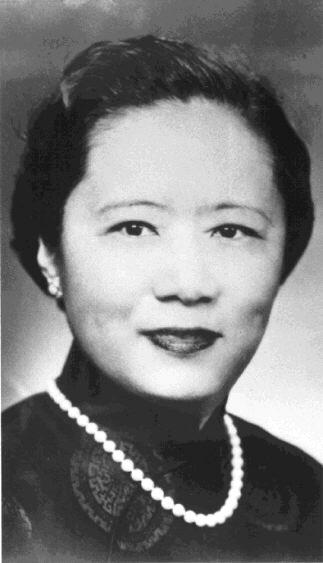
\includegraphics[width=0.3\textwidth]{fig/C_P_CP/Wu.jpg}
}&
\parbox{0.66\textwidth}{\textsf{\small
    ``Chien-Shiung Wu (often called "Madame Wu"), was born in Shanghai, China, in 1912. She
    received her Bachelor of Science degree in China in 1934 and came
    to the United States in 1936. After receiving her Ph.D. from the
    University of California in 1940, she taught at Smith College and
    at Princeton University before going to Columbia University in
    1944. As a nuclear physicist Dr. Wu worked on the Manhattan
    Project during the second World War. She became a professor of
    physics at Columbia and later held honorary professorships at
    several Chinese Universities. Dr. Wu received numerous honors and
    awards, including being the first woman elected president of the
    American Physical Society. She died in New York in February 1997.'' 
}}
\end{tabular}
\\  \textsf{Source: \httplink{http://www.physics.nist.gov/GenInt/Parity/people/Wu.html}}
\end{figure}
 Shortly after Young and Lee's proposal to search for parity violation in weak interactions, C.~S.~Wu, E.~Ambler, R.~W.~Hayward, D.~D.~Hoppes and
 R.~P.~Hudson showed in their
 \href{http://link.aps.org/abstract/PR/v105/p1413}{famous experiment}
 that parity is indeed
 violated\footnote{\href{http://link.aps.org/abstract/PR/v105/p1413}{C.S.~Wu, 
     E.~Ambler, R.W.~Hayward, D.D.~Hoppes and
     R.P.~Hudson Phys.~Rev.~{\bf 105},~1413~(157)}}.
\begin{figure}
\caption{Wu's Experiment}
\begin{tabular}{cc}
 Schematic & Not Wu \\
\parbox{0.49\textwidth}{
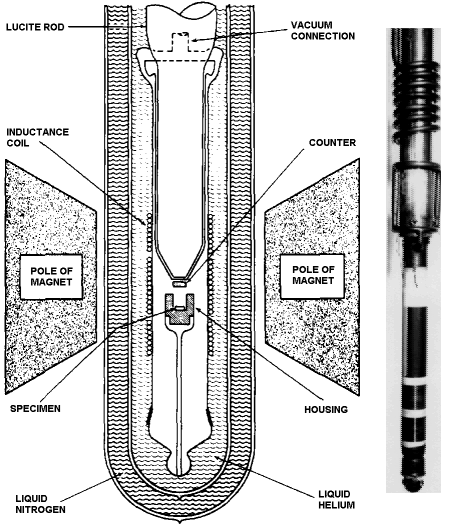
\includegraphics[width=0.49\textwidth]{fig/C_P_CP/wus_parity_apperatus.png}
}
&
\parbox{0.49\textwidth}{
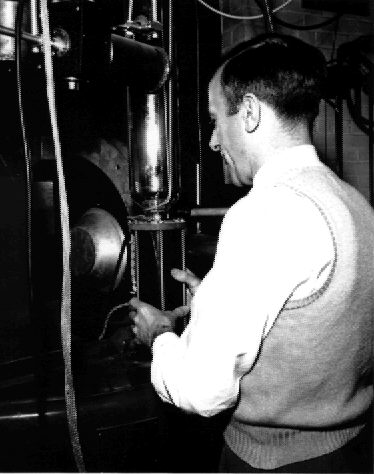
\includegraphics[width=0.49\textwidth]{fig/C_P_CP/wus_parity_photo.jpg}
}
\end{tabular}
\\Source:\href{http://physics.nist.gov/GenInt/Parity/expt.html#fig5-4-7}{\texttt{http://physics.nist.gov/GenInt/Parity/expt.html\#fig5-4-7}}
\end{figure}
 In the experiment, a sample of \chem{\mbox{}^{60}Co} is cooled down to
 very low temperatures, in a high magnetic field, and observed as it
 decays to \chem{\mbox{}^{60}Ni} under the emission of an electron and
 an (anti) neutrino. The observation was that the electrons were
 predominantly emitted opposite to the direction of the magnetic
 field. 
 %%
\begin{figure}
\centering
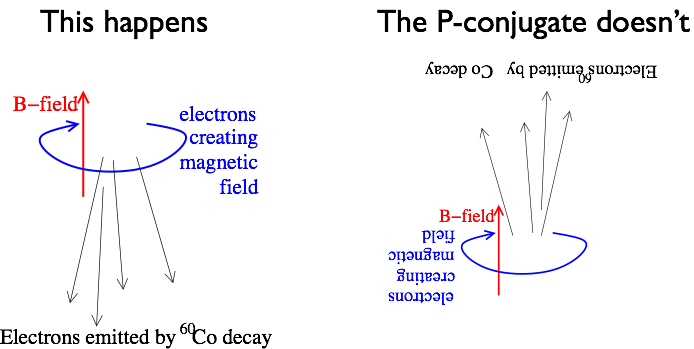
\includegraphics[width=0.8\textwidth]{fig/C_P_CP/0_MadamWuSchematic}
\caption{Schematic of Wu's experiment and how its P-conjugate would look like. Note that $\vec{B}$ does not change under \ps, while the momenta $\vec{p}$ do. So any momentum that is (always, or just preferentially) aligned with a $\vec{B}$ field must be \ps-violating. This is of course a simplified picture. In the real experiment, there would also be \emph{some} electrons that move in the other direction, along the $\vec{B}$ field (upwards in the picture on the left). This is because it is practically impossible to completely align the spins of the nuclei. But the observation of a significant up-down asymmetry in the electron direction is sufficient to prove \ps\ violation.
\label{fig:WuSchematic}}
\end{figure}
%%
\begin{figure}
\centering
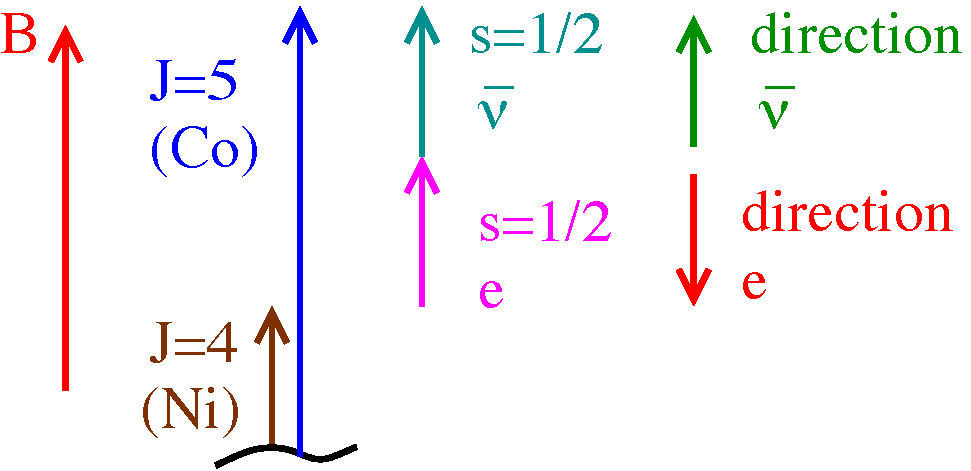
\includegraphics[width=0.8\textwidth]{fig/C_P_CP/0_MadamWuInterpretation}
\caption{Interpretation of Wu's experiment: The data can be explained if only (or at least preferentially) particles with negative helicity (spin opposite to the direction of motion, "left-handed particles") and anti-particles of positive helicity (right-handed particles) take part in the weak interaction. The true interpretation is not based on helicity, but the related, Lorentz-invariant quantity chirality.
\label{fig:WuInterpretation}}
\end{figure}
%%


\subsection{Helicity/Chirality}
%%%%%%%%%%%%%%%%%%%%%%%%
 We need something in the theory of weak interaction that violates
 parity, and Wu's experiment suggests, that this element has something
 to do with helicity (see \figref{fig:WuInterpretation}. The magnetic field aligns (approximately) the nuclear spins. The $L$ value the \chem{Ni} nuclues is one unit less than that of the \chem{Co} nucleus. Angular momentum conservation (more precisely the conservation of $L_z + S_z$) forces the spins of the electron and the anti-neutrino to align with the spin of the \chem{Co}, and hence the magnetic field.
 If predominantly (or only?) helicity
 right-handed anti-neutrinos, and helicity left-handed electrons participate in the interaction, the anti-neutrinos go (predominantly) in the direction of the field (upwards) and the electron to go (predominantly) downwards.
 
 So, one idea could be to make
 a theory where only those participate, i.e. the weak interaction only
 applies to helicity left-handed particles and helicity right-handed
 antiparticles.

 This is only \emph{nearly} the answer.

 The reason this does not quite work is that helicity is not Lorentz
 invariant. What's one observer's left-handed (massive) particle is
 another observer's right-handed one. Just imagine you see a helicity
 left-handed particle passing by - and a train that's travelling faster
 than that particle. If you change frames by jumping on that train,
 you'll find that the spin of the particle remains the same, but the
 velocity flips, so the helicity is now right-handed.  But a decay
 that happens in one frame of reference must also happen in
 another.

 So helicity can't be the distinguishing factor, but seems to have
 something to do with it. And it would work for zero-mass particles,
 that travel with the speed of light - you can't over-take a particle
 that travels at the speed of light, therefore they have the same
 helicity in all frames.

 The solution to the problem is called chirality. Chirality is Lorentz
 invariant. It is defined such that it is equivalent to helicity for
 zero-mass particles (see table \ref{tab:helichi} for details), but
 different for massive particles.

 Strictly only chirality left-handed particles take part in the weak
 interaction. For massless particles, this corresponds to helicity
 left-handed matter particles and helicity right-handed antimatter
 particles.

 The probability that a massive particle with definite chirality, e.g. an electron
 emerging from a weak decay which is definitely chirality
 left-handed, is found in the 'wrong', or suppressed
 helicity state is related to the followin matrix element
\begin{eqnarray}
\label{eq:wrongHeliProb}
\lefteqn{ \braket{\mathrm{e^-\;right-handed\;helicity}}{\mathrm{e^-\;left-handed\;chirality}}} \nonumber\\
 &\propto \frac{1}{2} \left(1 - \frac{|\vec{p}|}{m+E} \right)
\end{eqnarray}
%%
\begin{table}
\caption{Helicity and Chirality for massless particles.  For massive
 particles with definite helicity, there is a
 contribution of the ``wrong'' chirality. This means for example that a helicity-right handed particle can still interact weakly, with a probability $\sim (1-\frac{|\vec{p}|}{E+m})^{2}$, which goes to $0$ for $E\gg m$.
\label{tab:helichi}}
\begin{tabular}{c|cc c}
           &  chirality & helicity        & weak-interaction\\
           & \multicolumn{3}{|c|}{\small(for massless particle)} \\
 matter    &  left-handed & left-handed   &   yes \\
 matter    &  right-handed & right-handed &   no  \\
antimatter &  left-handed  & right-handed &   yes \\
antimatter &  right-handed & left-handed  &   no \\
\end{tabular}
\end{table}
%%
 For ultra-relativistic particles implying $E\gg m$, i.e. relative to
 their energy, they are nearly massless, helicity and chirality are
 essentially equivalent. For particles at rest on the other hand, a
 chirality left-handed particle at rest has a 50\%-50\% probability of
 being helicity left-handed or right-handed (well, for a particle
 really at rest helicity is not so well defined, imagine a particle
 that's moving very very slowly).

 Under the operation \ps, both chirality and helicity change sign.

 So the \ps\ violation in the weak interaction is pretty massive - the
 formal sentence is \textbf{``parity is maximally violated in the weak
 interaction''}. A massless particle that is subject to the weak interaction is, after
 applying the parity operator, suddenly not subject to it anymore at
 all.
 %\footnote{For massive particles the situation is a little more complicated, as it turns out that massive particles cannot be, at the same time, mass eigenstates and chirality eigenstates - and since it's mass eigenstates what we consider physical "particles", massive particles are always an admixture of chirality left and righthanded, but this admixture can be very unbalanced.}

\subsection{Intermezzo: Fermi's Golden Rule for particle decays}
In the section after this, we will discuss the decay of the pion and find out how parity violation has a profound effect on it. 
\begin{figure}
\centering
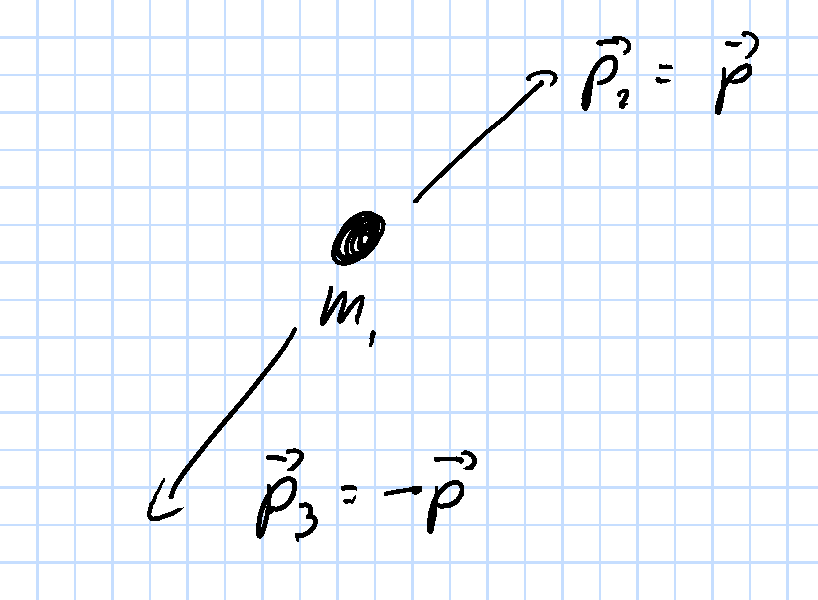
\includegraphics[width=0.4\textwidth]{fig/weak/Decay122}
\caption{Decay rate of particle $1$ into two particles (labelled $2$ and $3$) in the cm frame.\label{fig:Decay122}}
\end{figure}
Let's prepare ourselves by looking a bit closer at the "Golden Rule" that relates $\mathcal{M}_{fi}$ and hence the Feynman rules to decay rates, taking into account phase space density. (More on "Golden Rules" can be found in \appref{sec:GoldenRulesAndDensityOfStates}.)
\paragraph{Golden Rule for Decay Rates in cm frame}
(see \figref{fig:Decay122})
Decay of particle $1$ to particles $2, 3$ in the cm frame 
\begin{equation}
\Gamma_k = \frac{S}{8\pi} \frac{|\vec{p}|}{m_1^2} \left|\mathcal{M}_{fi}\right|^2
\end{equation}
Where $m_1$ is the mass of the decaying particle, and $\vec{p}$ is momentum of one of the daughter particles, $\vec{p} = \vec{p}_2 = -\vec{p_3}$. The subscript $k$ in $\Gamma_k$ indicates that this is the \emph{partial} width for the decay to this particular final state (that we label $k$). $S$ is $1$ when the final state particles are distinguishable (as in \prt{\pi^+ \to \mu^+ \nu_{\mu}}), except when the two final state particles are identical (as in \prt{\pi^0 \to \gamma \gamma}), in which case $S = \half$.
This is what you can do with the result of this calculation:
\begin{itemize}
\item $\Gamma_k$ is the partial width of the decay of particle $1$ to particles $2, 3$.
\item If I add up all partial widths (i.e. $\Gamma_k$ calculated for all possible final states $k$, added together) I get the total width $\Gamma = \sum_k \Gamma_k$. Its inverse is the average lifetime of the particle, $\tau = 1/\Gamma$. If I start with $N_0$ particles, I expect, after time $t$ (in the particles' restframe), to find $N(t) = N_0 e^{-\Gamma t}$.
\item If we have $N$ particles, the rate at which they will decay to this given final state is $N\Gamma_k$ (note that $N$ will decrease exponentially with time, $N(t) = N_0 e^{-\Gamma t}$).
\item If I observe $n$ decays of this given type of particle, the fraction of decays $n_k$ that I expect to find in final state $k$ is $n_k/n = \Gamma_k/\Gamma$. This ratio is called the Branching Fraction.
\end{itemize}
\paragraph{Phase Space Density}
Apart from some constants, the key factor that we find in addition to $\mathcal{M}_{fi}$ (which we get from Feynman rules) is the magnitude of the three-momentum of the daughter particles in the restframe of the mother, $|\vec{p}|$. This takes into account the number of different quantum mechanical states with (nearly [never forget Heisenberg's uncertainty principle]) the same momentum $|\vec{p}|$ that the final state can occupy - the decay rate is directly proportional to this. This proportionality factor is usually referred to as "phase space factor" or "phase space density". It is derived in \appref{sec:densityOfStates}. 
For the case of a decay of a particle with mass $M_A$ to two particles with masses $m_B, m_C$, the phase space factor is given by
\begin{equation}
\label{eq:phsp_dens}
 |\vec{p}| = \frac{\sqrt{(M_A^2 - (m_B + m_C)^2)(M_A^2 - (m_B - m_C)^2)}}{2M_A}
\end{equation}
Note that such a phase space factor applies no matter how the final state came about, by the decay of a particle, or through scattering. 
In the latter case, $M_A$ is replaced by the $cm$ energy. In either situation, when calculating ratios of rates, it only matters if the decay product are not much lighter than the mother particle / the collision energy. For $M_A \gg m_B, m_C$, this reduces to a constant ($\half M_A$) that cancels when calculating decay rate ratios. For example the phase space factor does not matter when calculating $R$ in \secref{sec:FormationOfJets}, because the collision energy is much higher than the masses of the quarks or leptons involved; it would also not matter when calculating ratios like $\Gamma(\prt{B^0 \to \pi^+ \pi^-})/\Gamma(\prt{B^0 \to K^+ K^-})$ because the $B^0$ meson is so much heavier than either pions or kaons. 
It will matter in the next section for the case where the pion decays to a muon and a neutrino. The muon's mass is very close to the pion's mass (this is why the muon, when it was discovered, was initially mistaken for the pion)\\
\fbox{\parbox{0.9\textwidth}{
\paragraph{We remember...}
\begin{itemize}
\item Fermi's Golden Rule relates Feynman rules and decay rates. Its key statement is:
$\Gamma_{f} \propto |\mathcal{M}_{fi}|^2 \times \mathsf{(phase-space-factor)}$.
\item The phase space factor takes into account the density of states and favours decays to lighter particles over decays to heavier particles.
\item When calculating ratios of rates with the same initial state, this phase space factor only matters if the mother particle's mass (or the collision energy) is not much higher than the masses of the decay products.
\end{itemize}
}}


\subsection{Pion decay} 
 Let us consider the ratio of decay rates of $\pi^- \to e^- \bar{v}_{e}$
 to $\pi^- \to \mu^- \bar{v}_{\mu}$. Naively, because of phase space
 considerations, one would expect the decay to the much lighter
 electron to dominate. However, the pion decays nearly always to the
 much heavier muon. Parity violation is the explanation.

 Due to angular momentum and momentum conservation, the two decay
 products of the $\pi$, which has spin 0, must have the same
 helicity. Assuming that the anti-neutrino is massless, and looking at
 table \ref{tab:helichi}, the anti-neutrino must have positive
 helicity. That leaves the electron or muon no choice but have
 positive helicity as well. But of course the electron/muon must also
 have negative chirality. From Eq.~\ref{eq:wrongHeliProb} we know that the probability
 to find a right-handed helicity lepton in a left-handed chirality state is
 proportional to
 \[
 \left(1-\frac{|\vec{p}|}{E+m}\right)^{2}
 \]
 For the two-body decay of the pion this expression reduces to
 \begin{equation}
 \label{eq:wrongHeliProbPion}
\left(\frac{m_{\ell}}{m_{\pi}+m_{\ell}}\right)^2
 \end{equation}
 where we used energy and momentum conservation to obtain the final expression
 ({\bf Problem Sheet 3})

\begin{figure}
\centering
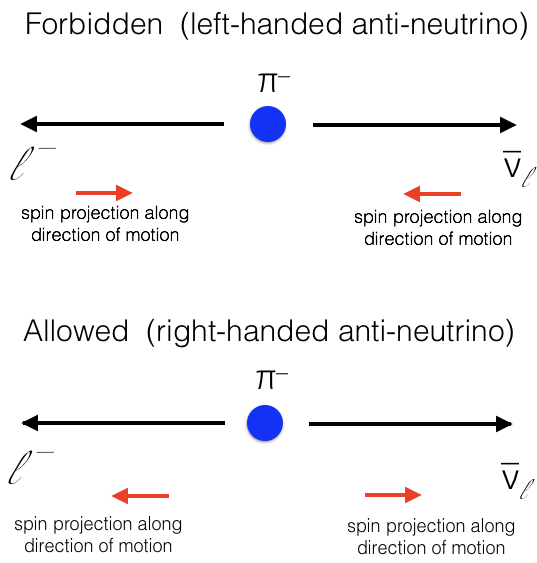
\includegraphics[width=0.6\textwidth]{fig/0_pionDecay}
\caption[Pion Decay]{Pion Decay: To conserve $\vec{L} + \vec{S}$, the spin-projections for the charged lepton ($\ell^-$) and the anti-neutrino have to be opposite, leading the the two possible configurations shown above. Since the neutrino is (nearly) massless, only the helicity right-handed anti-neutrinos interact, while helicity left-handed anti-neutrinos do not.
\label{fig:my_label}}
\end{figure}

 From Eq.~\ref{eq:wrongHeliProbPion} we can estimate the ratio of
 decay rates, neglecting phase-space effects. Let's start with the
 decay to electrons: Compared to the pion, the electron is very 
 light so the probability of it interacting with the suppressed
 helicity is
\begin{equation}
 \sim \frac{m_e^2}{m_{\pi}^2}
\end{equation}
 Now the muon has nearly the same mass as the pion. So
 the probability for it to have the suppressed helicity is
\begin{equation}
 \sim \frac{m_{\mu}^2}{4 m_{\mu}^2} = \frac{1}{4}
\end{equation}
 and the ratio between the two:
\begin{equation}
 \sim 4\frac{m_e^2}{m_{\pi}^2} \sim 5\cdot 10^{-5},
\end{equation}
 massively favouring the decay to the muon.
 On the other hand, the phase space factor
 \begin{equation}
 \Phi \propto |\vec{p}| = 
 \frac{m^2_{\pi} - m^2_{\ell}}{2 m_{\pi}}
 \end{equation}
(where $\ell$ is either the electron or the muon) favours the decay to the electron. Combining the two competing contributions gives an estimate of the decay rate ratio of
 \begin{equation}
 \frac{\Gamma(\pim \to e^- \overline{\nu}_e)}{
    \Gamma(\pim \to \mu^- \overline{\nu}_{\mu})}
\sim
 4\frac{m_e^2}{m_{\pi}^2} 
    \left(
     \frac{m^2_{\pi} - m^2_{e}}{
     m^2_{\pi} - m^2_{\mu}}
    \right)
 \sim 1.2\cdot 10^{-4}
\end{equation}


 The full calculation can be found in many text
 books and leads to a slightly different expression
 including an additional factor of 
 $\frac{1}{4}\left(
     \frac{m^2_{\pi} - m^2_{e}}{
     m^2_{\pi} - m^2_{\mu}}
    \right)$. 
The result is
\begin{equation}
 \frac{\Gamma(\pi \to e \nu_e)}{\Gamma(\pi \to \mu \nu_{\mu})}
=
\frac{m_e^2}{m_{\mu}^2} \left(\frac{m^2_{\pi} - m^2_{e}}{m^2_{\pi} -
  m^2_{\mu}}\right)^2
= 1.23 \cdot 10^{-4}.
\end{equation}

So, due to the \ps-violation-induced \emph{helicity suppression}, the pion decay to the muon completely dominates over the decay mode to the electron (and in fact anything else, so charged pions essentially always decay to muons and (anti) muon neutrinos). This is the opposite of what one would expect without helicity suppression, where the electron mode would dominate because of phase space considerations. This result is in excellent agreement with the experimental value for the decay rate ratio of $(1.230\pm 0.004) \cdot
 10^{-4}$. 
A rather striking effect of \ps\ violation.

\section{\cs{}harge Conjugation}
\label{sec:ChargeConjugation}
 The Charge conjugation operator transforms particles to
 antiparticles. Like for the parity operator, it follows from $\cs^2=1$
 that it can have the eigenvalues $+1$ and $-1$.

 It is called 'charge conjugation' because it swaps all charges -
 positive and negative electric charge as well as colour charge (for
 the strong interaction) and weak charge. \cs\ also swaps the
 chirality quantum number (but not the helicity quantum number, but as
 you can see from table \ref{tab:helichi}, as far as the weak
 interaction is concerned, the effect is the same).

 Neutral particles can be (but don't have to be) \cs\
 eigenstates. Charged particles of course cannot. However,
 particle-antiparticle pairs of charged (or neutral) particles can
 also be \cs\ eigenstates (they might even have been created in the
 decay of a \cs\ eigenstate).

 Like \ps, \cs is a multiplicative quantum number. For a system of
 particles with well-defined C-parity the total \cs\ eigenvalue is the
 intrinsic \cs\ eigenvalues of the particles involved. 

 If the particles involved are not themselves parity eigenstates, but
 particle-antiparticle pairs, the C-parity number is given by a factor
 that derives from the behaviour of the total wavefunction under the
 exchange of particles, and is therefore different for fermions pairs
 and for boson pairs. For a pair of bosons (like $\pi^+\pi^-$ or
 $\gamma, \gamma$), C parity is $(-1)^{L}$, where $L$ is the angular
 momentum of the pair. For pairs of spin-\half fermions (like $e^+,
 e^-$), the factor is $(-1)^{L+S}$, where $S$ is the total spin
 quantum number of the system.

 The quantum numbers of particles are usually given in the following
 format:
\begin{equation}
%
  J^{(PC)} \;\;\;= \;\;\;\mbox{Spin}^{(\mathrm{parity,\;\; \cs-eigenvalue})}
%
\end{equation}
 The $J^{(PC)}$ of some important particles are:\\
\begin{tabular}{|*{7}{c|}}
\hline
 $\gamma$ & $\pi^0$ & $\pi^{\pm}$ & $K^0$   & $K^{\pm}$ & p & n
\\\hline
 $1^{--}$ & $0^{-+}$& $0^{-}$     & $0^{-}$ & $0^{-}$   & $\half^{+}$
 & $\half^{+}$
\\
\hline
\end{tabular}

For a system of $C$-eigenstates:
\[
\prod\limits_{\mathsf{all\;particles}}
\mbox{(intrinsic C)}
\]
For a particle anti-particle pair of bosons that are not $C$
eigenstates (e.g. $\pi^+\pi^-$):
\[
C = (-1)^L
\]
This is a consequence of the fact that here, \cs has the same effect as \ps.
For a fermion-antifermion pair (e.g. $e^+ e^-$) it's a bit more complicated, we have to account for the behaviour of the wave function under spin exchange. For relative angular momentum $L$ and and total spin $S$:
\[
C = (-1)^{L+S}
\]




